\begin{figure}[H]
\centering
\includegraphics[page=6,width=0.48\textwidth]{\FCNCFigures/xTFW/raw/NOMINAL/reg2mtau1b2jos_vetobtagwp70_highmet/tau_pt_0.pdf}
\put(-100, 140){\textbf{(a1)}}
\put(-120, 130){\footnotesize{STH $\thadhad$ (OS)}}
\includegraphics[page=6,width=0.48\textwidth]{\FCNCFigures/xTFW/raw/NOMINAL/reg2mtau1b3jos_vetobtagwp70_highmet/tau_pt_0.pdf}
\put(-100, 140){\textbf{(b1)}}
\put(-120, 130){\footnotesize{TTH $\thadhad$ (OS)}}\\
\includegraphics[page=6,width=0.48\textwidth]{\FCNCFigures/xTFW/raw/NOMINAL/reg2mtau1b2jss_vetobtagwp70_highmet/tau_pt_0.pdf}
\put(-100, 140){\textbf{(a2)}}
\put(-120, 130){\footnotesize{STH $\thadhad$ (SS)}}
\includegraphics[page=6,width=0.48\textwidth]{\FCNCFigures/xTFW/raw/NOMINAL/reg2mtau1b3jss_vetobtagwp70_highmet/tau_pt_0.pdf}
\put(-100, 140){\textbf{(b2)}}
\put(-120, 130){\footnotesize{TTH $\thadhad$ (SS)}}
\caption{ The distributions of leading $\tau$ $\pt$ in the STH (a), and TTH (b) $\thadhad$ SR (1) and SS CR (2) before the fake estimation. Data is more than the MC prediction because the fake tau backgrounds are not yet added.}
\label{fig:os_pre_hadhad}
\end{figure}
